\problemname{Brevoptimering}
Progolympkommittén, bestående av $N$ personer, ska skicka ut kuvert med affischer för kvalet till alla skolor.
För att göra processen snabbare har de delat upp uppgifterna som behöver göras.
Uppgifterna är bland annat att skriva adresser, sätta på frimärken, lägga i affischerna och stänga kuverten.
När en person är klar med ett kuvert skickas det vidare till någon annan person.
Det går inte lika snabbt som de hade hoppats på, och därför undrar de vilka som skulle kunna jobba snabbare.

Varje person $p$ har en egen maximal produktionshastighet $M_p$ kuvert per sekund.
Om vi låter $I_p$ vara antalet kuvert som skickas till person $p$ per sekund och låter $U_p$ vara antalet kuvert den blir klar med per sekund så är $U_p = \min(I_p, M_p)$.
En person blir alltså inte klar med fler än $M_p$ brev per sekund, även om hen får fler att arbeta med.
Varje person har dessutom att antal personer den skickar de kuvert hen blir klar med.
Den behöver inte skicka lika mycket kuvert till varje person, utan varje person får en viss procent av kuverten $p$ skickar.
De personer som ingen skickar kuvert till och som därmed är i början av produktionslinjen har $I_p = \infty$, och därmed $U_p = M_p$ (de har en oändlig hög med kuvert att ta av).
Vissa personer skickar inte vidare några kuvert alls, utan lägger dem bara i hög bredvid sig när de är klara.

För vilka personer gäller att $U_p = M_p$, det vill säga att de jobbar på sin maximala produktionshastighet?

\section*{Indata}
Den första raden innehåller ett heltal $1 \le N \le 10^5$, antalet personer.
De nästa $N$ raderna beskriver personerna. Rad $i$ innehåller först heltalet $M_i$, den maximala produktionshastigheten för person $i$ ($1 \le M_i \le 10^5$).
Därefter kommer ett heltal $k$, och sedan $k$ par av heltal $j$ $w$, som betyder att person $i$ skickar $w$ procent av sina kuvert till person $j$ ($1 \le w \le 100$, $1 \le j \le N, i \neq j$).
Inget $j$ kan förekomma mer än en gång på en given rad, och summan av $w$:na på raden kommer att vara $100$, såvida inte $k = 0$.

Låt $S$ beteckna summan av alla $k$. Då gäller $0 \le S \le 10^5$.

Produktionskedjan är designad på ett sådant sätt att ingen person kan få tillbaka ett brev de redan arbetat med.

\section*{Utdata}
Skriv ut en rad med alla $i$ som uppfyller $U_p = M_p$, i stigande ordning.

Det garanteras att om $U_p = M_p$ så kommer detta stämma med marginal, mer specifikt $I_p - M_p > 10^{-4}$.
Om tvärt om $U_p \neq M_p$ så kommer det finnas marginal åt andra hållet: $M_p - I_p > 10^{-4}$.

\section*{Poängsättning}
Din lösning kommer att testas på en mängd testfallsgrupper.
För att få poäng för en grupp så måste du klara alla testfall i gruppen.

\noindent
\begin{tabular}{| l | l | l |}
\hline
Grupp & Poängvärde & Gränser \\ \hline
$1$    & $12$       &  Varje person skickar brev till högst en person (d.v.s $k \leq 1$) och tar emot brev från max en person \\ \hline 
$2$    & $17$       &  Varje person tar emot brev från exakt en annan person, förutom person $1$ som inte tar emot från någon \\ \hline 
$3$    & $21$       &  Om person $i$ skickar till person $j$ så är $i < j$ \\ \hline
$4$    & $25$       &  $N, S \le 10$ \\ \hline
$5$    & $25$       &  Inga ytterligare begränsningar. \\ \hline
\end{tabular}

\section*{Förklaring av exempelfall}
Här följer tre grafer som representerar de tre exempelfallen. Varje person representeras av en nod. På varje kant är mängden kuvert som skickas utskrivet i enheten kps, kuvert per sekund.

Notera att i testfallsgrupp $1$ skulle enbart exempelfall $1$ kunna förekomma, i testfallsgrupp $2$ enbart exempelfall $2$, och i testfallsgrupp $3$ enbart exempelfall $3$.
I testfallsgrupp $4$ och $5$ skulle alla tre exempelfall kunna förekomma.
\begin{figure}
	\centering
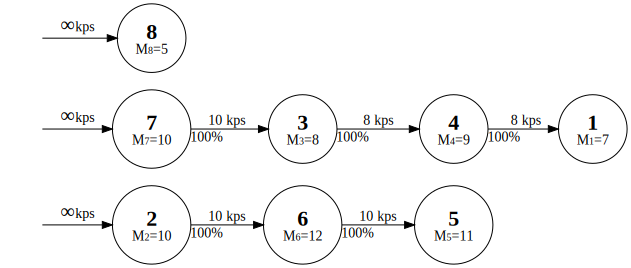
\includegraphics[width=0.8\textwidth]{sample1}
\caption{Sample $1$}
\end{figure} 
\begin{figure}
	\centering
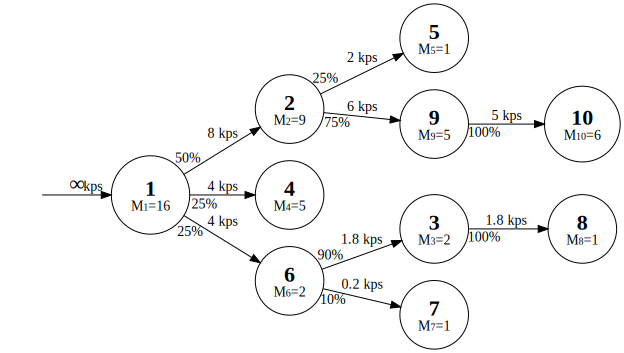
\includegraphics[width=0.8\textwidth]{sample2}
\caption{Sample $2$}
\end{figure} 
\begin{figure}
	\centering
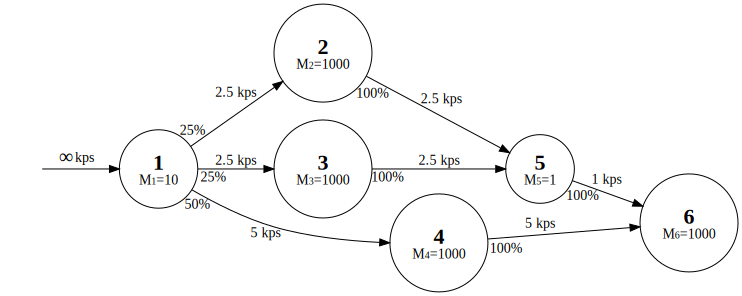
\includegraphics[width=0.8\textwidth]{sample3}
\caption{Sample $3$}
\end{figure} 
